\section{Aktivitetsmålere til børn} \label{tracker_intro}
%%Den gamle intro
%\textit{Dette afsnit omhandler, en beskrivelse af funktionaliteten for en række udvalgte aktivitetsmålere. Disse aktivitetsmålere bliver vurderet og analyseret på baggrund af opstillede succeskrav. Afslutningsvis præsenteres den samlede vurdering af aktivitetsmålerne, og hvordan disse opfylder opstillede kriterier.}
\textit{Dette afsnit omhandler optimale egenskaber for en aktivitetsmåler samt funktionaliteten af nuværende aktivitetsmålere til børn. På baggrund af dette analyseret en række nuværende teknologier, samt vurderes med henblik på at kunne designe en teknologi der opfylder succeskriterier på bedst mulig vis.}
%%Gammel indledning 
%
%Sundhedsstyrelsen anbefaler børn at motionere 2,5 ugentligt, hvis dette ikke opfyldes karakteriseres barnet som inaktivt. Manglende motion kan være som resultatet af den teknologiske udvikling, som medfører en mere stillesiddende livsstil. \citep{ObesityActionCoalition} Den teknologiske udvikling som medvirker til inaktivitet og stillesiddende livsstil, er forsøgt udnyttet som modarbejdende faktor. Flere producenter har benyttet teknologi som et led i at motivere børn til et mere aktivt liv \citep{Fuhu2015,PowerAbout2015}. Fælles for disse producenter er, at de motiverer børn til at fysisk aktivitet gennem spil og leg. Producenterne benytter aktivitetsmålere til at registrere aktivitet. Sideløbende belønnes børnene med et antal point, afhængigt af aktivitetsniveauet. Børnene har i mange tilfælde mulighed for at spille alene, men også i hold. Dette medfører en mulig implementering af motions motiverende teknologier i et skoleregi. \newline
%Potentialet af en teknologi som motiverer børn til en aktiv livsstil kan have flere fordele. Den primære fordel ved en aktiv livsstil er forebyggelsen af følgesygdomme. Dette har vist sig at være en fordelagtig økonomisk og sundhedsmæssig investering.
%% Ny indledning

\subsection{Aktivitetsmålere}
Aktivitetsmålere kan benyttes af alle aldersgrupper til at registrere det fysiske aktivitetsniveau. Den kan registrere data for en bestemt dag eller over en længere periode. Aktivitetsmålere benytter en eller flere sensorer til at registrere det fysiske aktivitetsniveau. Eksempelvis kan et pedometer, accelerometer eller gyroskop findes i en aktivitetsmåler. Et pedometer kan bestemme antal skridt via en svingende pendul hammer i et kredsløb. Mere moderne pedometre benytter accelerometre, der vinkelret på hinanden kan detektere skridt. Et accelerometer måler acceleration i m/s$^2$ eller g-kræfter, hvilket er et udtryk for tyngdepåvirkningen af sensoren under bevægelse. Et gyroskop måler vinkelhastighed i $^\circ$/s eller omdrejninger pr sekund. Dette kan anvendes til at bestemme orientering eller balanceinformation. \citep{Sparkfun,Woodford2016,Sparkfun_gyro} \newline
Et fælles formål for aktivitetsmålerne er dermed at bestemme det fysiske aktivitetsniveau gennem en række analoge og digitale elementer. De digitale elementer benyttes til at bestemme og visualisere sensorens opsamlede data. Dermed er de digitale elementer blandt andet bestemmende for den brugerflade, som er tilhørende den pågældende aktivitetsmåler. En aktivitetsmåler, som er specifikt designet til børn, har muligvis en brugerflade, som involverer spil og leg for at motivere barnet til øget fysisk aktivitet. 

\subsection{Succeskriterier for aktivitetsmålere} \label{succeskrav}
Flere producenter har benyttet teknologi, som et led i at motivere børn til et mere aktivt liv gennem spil og leg ved hjælp af aktivitetsmålere. Børnene har i mange tilfælde mulighed for at spille alene eller sammen med andre. %, hvorfor det er muligt at implementere aktivitetsmotiverende teknologier i et skoleregi. 
\citep{Fuhu2015,PowerAbout2015} %Denne sammenkobling af teknologi og fysisk aktivitet er blandt andet udnyttet af firmaet Playware, som har haft positive resultater hvad angår motivering til øget fysisk aktivitetsniveau \citep{Rishoej2010}. \newline% Yderligere giver frivillig fysisk aktivitet med intrinsisk motivation det bedste udbytte for børn \citep{J.Sebire2013}. \newline
En teknologi, som motiverer børn til en aktiv livsstil, har potentielt flere samfundsøkonomiske og sundhedsmæssige fordele, idet en aktiv livsstil blandt andet er forebyggende for diverse følgesygdomme, som beskrevet i \secref{subsec:inover}.

Aktivitetsmålere til børn bør tage højde for en række essentielle kriterier, som blandt andet indebærer, at alt barnets daglig aktivitet registreres. Dermed skal systemet registrere og gemme al aktivitet igennem et barn hverdag, hvilket indebærer både skoleaktiviteter såvel som fritidsaktiviteter. I og med al fysisk aktivitet registreres vil der dannes en mere realistisk gengivelse af barnets aktivitetsniveau. \\%skal barnets samlede fysisk aktivitet i løbet af en dag, indeholdene fritidsaktiviteter såvel som skolerelaterede aktiviteter, kunne registreres og gemmes af systemet.  %Nævnt i \secref{subsec:fysio_aktivitet} anbefales det, at børn dagligt udfører 60 minutters aktivitet med moderart til høj intensitet. 
Et studie har undersøgt, hvilke børneidrætter der er de 10 mest populære blandt børn i aldersgruppen 7-15 år. Det fremgår af dette studie, at 7 ud af de 10 mest populære børneidrætter involverer gang eller løb \citep{Asserhoej2013}. Desuden fremgår det af flere  studier, at cykling er en af de hyppigst benyttede transportmidler for børn i alderen 10-15 år \citep{DTU2014,COWI2015}. På baggrund af dette skal en aktivitetsmåler kunne registrere gang, løb og cykling for dermed at kunne bestemme barnets samlede fysiske aktivitetsniveau i løbet af en dag. Ydermere skal aktivitetsmåleren kunne skelne mellem disse aktivitetsformer. Denne automatiske genkendelse kan udformes ved brug af flere forskellige sensorer. Herved kan aktivitetsmåleren opnå en stor brugervenlighed, idet barnet ikke selv skal indtaste, hvilken type aktivitet der vil blive udført. \newline
Intensiteten af en given fysisk aktivitet kan bestemmes af en persons puls, som det fremgår i afsnit \secref{subsec:fysio_aktivitet}. Det vil derfor være fordelagtigt, hvis aktivitetsmåleren kan bestemme barnets puls og herigennem kategorisere intensiteten samt den fysiske effekt af aktiviteten.
%
%Idet aktivitetsmåleren skal anvendes igennem en skoledag, så skal aktivitetsmåleren også kunne registrere aktivitetsformer, der er tilgængelige i skolen. Sundhedsstyrelsen har opstillet en række aktivitetsformer, hvor det ønskede intensitetsniveau opnås. Aktivitetsformer, som er tilgængelige for børn igennem en skoledag, er eksempelvis lege, der indebærer løb, leg i skolegården, cykling, fodbold og basketbold. Fælles for disse aktivitetsformer er, at de kan registreres som gang, løb og cykling. \citep{Sundhedsstyrelsen2003}
%I takt med at den daglige aktivitet opfanges bør en aktivitetsmåler kunne registrere, og dermed også adskille, gang, løb og cykling, hvilket gøres gennem forskellige sensorer.
%
%For at en aktivitetsmåler kan registrere aktivitet, kræves det at aktivitetsmåleren indeholder sensorer. Med den rette algoritme kan sensorer automatisk skelne mellem de nævnte former for aktivitet. 
%Idet de fysiologiske effekter i forbindelse med aktivitet er forskellige alt efter intensitetsniveauet, skal aktivitetsmåleren ydermere kunne registrere intensiteten af aktiviteten og belønne brugeren gennem brugerfladen.  

Målgruppen for den tilsigtede aktivitetsmåler er børn i aldersgruppen 9-12 år. Det er påvist, at børn i denne aldersgruppe motiveres bedst gennem frivillig fysisk aktivitet med intrinsisk motivation som leg og spil. Aktivitetsmåleren skal derfor kunne benytte sig af en type motivation, som henvender sig til målgruppens behov.

Aktivitetsmålerens placering og påmontering skal desuden være komfortabel. Aktivitetsmåleren må ikke fratage eller hindre barnets psykiske eller fysiske udfoldelse i forbindelse med afbenyttelse. 
%Da aktivitetsmåleren skal benyttes hovedsageligt af inaktive børn, skal den kunne motivere til fysisk aktivitet. Ifølge \secref{motivation_boern} tyder det på, at børn i den udvalgte målgruppe motiveres til aktivitet gennem leg og spil. Et essentielt kriterie vil derfor være at kunne motivere denne målgruppe uanset alder og køn. \newline
%En aktivitetsmåler skal ikke være til gene, da en eventuelt gene i forbindelse med placeringen muligvis vil medføre fravalg af benyttelse og derved fysisk aktivitet. Derfor er et yderligere kriterie, at aktivitetsmåleren ikke skal være til gene. Børnene med en aktivitetsmåler påsat skal være lige så frie som foruden.

Den optimale aktivitetsmåler skal dermed kunne: 
\begin{itemize}
\item Registrere gang.
\item Registrere løb.
\item Registrere cykling. %Når de står registreret hver for sig, så menes der derved, at de kan skelnes fra hinanden.
\item Registrere aktivitetens intensitet. %igennem puls
\item Motivere både fysisk inaktive og fysisk aktive børn. %socialt
\item Monteres og placeres på komfortabel vis.
\end{itemize}

\subsubsection{Afgrænsning af aktivitetsmålere}  %Hed før Baggrund for analyse og vurdering af aktivitetsmålere
Der er udvalgt fire aktivitetsmålere til videre analyse, som alle har samme formål; at motivere børn til et øget fysisk aktivitetsniveau. De udvalgte aktivitetsmålere henvender sig alle til børn i målgruppen 9-12 år og har derfor på forskellig vis udformet en brugerflade, som er motiverende for målgruppen. Ydermere er aktivitetsmålerne trådløse og tilbyder en brugerflade gennem trådløs overførsel i form af en hjemmeside og/eller app. \newline
De udvalgte aktivitetsmålere vil blive analyseret og vurderet på baggrund af ovenstående succeskriterier.

\subsection{UNICEF kid power band}
UNICEF Kid Power Band er en aktivitetsmåler, som appellerer til børn ved at hjælpe andre børn i ressourcefattige lande, hvoraf sloganet til aktivitetsmåleren lyder: "Vær aktiv. Red liv".
Aktivitetsmåleren, der er udformet som et armbånd, fremgår af~\figref{fig:unicef}. Aktivitetsmåleren benytter et pedometer og et accelerometer til at registrere barnets fysiske aktivitet. Det opsamlede data overføres trådløst til en app, som kan hentes ned på enheder med bluetooth. \citep{PowerAbout2015,PowerManual2015}

\begin{figure}[H]
	\centering
	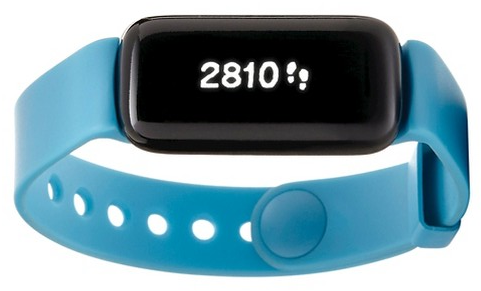
\includegraphics[scale=0.55]{figures/aProblemanalyse/unicef.png}
	\caption{På figuren ses UNICEF kid power band. \cite{Unicef2016}}
	\label{fig:unicef}
\end{figure}
Børnene kan optjene point ved at være fysisk aktive. Der optjenes point efter, hvor fysisk aktive børnene er. Pointene omregnes til en sum penge, som sponsoreres af fans, firmaer og forældre. Pengene, som børnene optjener igennem fysisk aktivitet, bliver doneret til ressourcefattige lande, som er en del af UNICEFs tiltag. %Pengene, som børnene dermed gør sig fortjent til gennem fysisk aktivitet, vil blive sendt til de ressourcefattige lande, som aktivitetsmåleren støtter. \newline
Børnene har mulighed for at vælge mellem en række udvalgte lande gennem missioner. Disse missioner skal lære børnene om samfundet i det pågældende land og give dermed børnene indsigt i, hvor betydningsfuld deres hjælp er. Børnene har gennemført en mission, når de har været tilstrækkeligt fysisk aktive til at optjene samtlige tilgængelige point. Alle resultater samles i en app, hvor børnene har mulighed for at følge med i progressionen for dem selv samt deres venner samt for de missioner, som de deltager i. Aktivitetsmåleren har en indkøbspris på 280 kr. \citep{PowerAbout2015,PowerManual2015}
%
%For at optjene point, skal børnene gennemføre forskellige missioner, som professionelle atleter står i spidsen for, hvorigennem børnene ikke blot er aktive men også lærer om forskellige kulturer.\fxnote{Et eksempel er en mission, som basketballspilleren Tyson Chandler står i spidsen for, hvor børnene lærer om hvordan børn i ressourcefattige lande, hjælper familien med at gro deres eget mad.} \citep{PowerMission2015} 
%Børnene kan selv følge med i, hvor langt de er i den pågældende mission på aktivitetsmåleren eller gennem en applikation (app). Når børnene har gennemført en mission, omregnes deres point til en sum penge, sponsoreret af fans, firmaer og forældre, som sendes til det pågældende ressourcefattige land, som missionen støtter. \newline
%Hver dag nulstilles aktivitetsmåleren, så børnene hver dag kan følge med i hvor aktive de har været den pågældende dag. Derudover gemmes der data 30 dage tilbage, så det er muligt at sammenligne med tidligere dage. 
%På aktivitetsmåleren er der en skærm, hvor det er muligt at følge med i klokken, antal skridt, KidPower points, fremskridt på missioner og navnet på brugeren. 
%Alle resultater samles i en applikation (app), hvor børnene både har mulighed for at følge med i progressionen for dem selv og deres venner, samt for de missioner de deltager i. \citep{PowerAbout2015}

\subsubsection{Vurdering af succeskriterier}
Aktivitetsmåleren's funktion er at tælle skridt, hvilket registreres under løb og gang, men der skelnes ikke mellem aktiviteterne. Idet armene ikke bevæges ved cykling, er denne aktivitetsform ikke mulig for måleren at registrere. Aktivitetsmåleren kan ikke registrere intensiteten af den målte aktivitet, idet der kun måles på, hvor energisk armen bevæges under en given øvelse og ikke puls, iltoptagelse eller anstrengelse. %Derudover måles intensitet af det udførte arbejde ikke, idet der udelukkende måles hvor energisk armene bevæges under en givne øvelse, og ikke puls, iltoptagelse eller anstrengelse. 
Aktivitetsmåleren er designet som et armbånd med en justerbar rem, hvilket gør at den kan monteres og placeres på komfortabel vis. \citep{PowerManual2015} \newline
Børnene udfører de fysiske aktiviteter sammen med andre børn med henblik på at hjælpe børn i ressourcefattige lande. Aktivitetsmåleren motiverer børnene på intrinsisk vis ved hjælp af de sociale aspekter, som ligger til grund for aktivitetsmålerens brugerflade.%Børnene aktiveres socialt, da alle aktiviteter udføres med henblik på at de sammen med jævnaldrende, skal hjælpe børn i ressourcefattige lande. Derudover bliver børnene gennem appen opdateret på progression i de missioner de deltager i, samt venners progression, hvorved det ikke kun er den individuelle præstation der er i fokus. %Flere skoler i USA har i fjerde klasse også benyttet aktivitetsmåleren, som en del af klasseprojekter, for at få børnene til at blive mere aktive. 
~\citep{PowerAbout2015} 

UNICEF Kid Power Band opfylder to ud af seks succeskriterier, mens det delvist opfylder to succeskriterier.

\subsection{The Sqord Booster}
The Sqord Booster er en aktivitetsmåler, som appellerer til børn i alderen 8-14 år gennem konkurrence og fællesskab. Aktivitetsmåleres motiverer børn igennem spil, hvor alt udført aktivitet gemmes i en avatar. Denne avatar designer børnene selv på en hjemmeside, hvor de også kan kommunikere med deres venner. Forældrene har mulighed for at oprette et forældrelogin til siden, så de ligeledes kan følge med i deres børns aktivitet. Aktivitetsmåleren er designet til at blive brugt i grupper men er ikke betinget af fysisk tilstedeværelse, da online gruppekommunikation også er muligt.% dette er dog uafhængigt af, om børnene fysisk eller online er sammen. 
~\citep{Sqord_family2015} Børnene kan enten konkurrere mod hinanden eller arbejde sammen som et hold. Det er også muligt at benytte aktivitetsmåleren individuelt, da barnet kan følge sin og andres udvikling. Hermed kan der opstå interne konkurrencer i forbindelse med barnets formåen. \citep{Sqord_family2015,Sqord_group2015} \\
Børnene optjener point ved at deltage i forskellige konkurrencer, hvor deres aktivitet måles gennem et tre-akse accelerometer. Det opsamlede data overføres trådløst til en app, som kan hentes ned på enheder med bluetooth low energy. Aktivitetsmåleren placeres oftest om håndleddet som et armbånd, hvilket kan ses på \figref{fig:sqord}. Aktivitetsmåleren kan også placeres i en lomme eller bundet til skoen angiveligt uden indflydelse på målingerne, som sensorerne udfører. \citep{Sqord_family2015}
\begin{figure}[H]
	\centering
	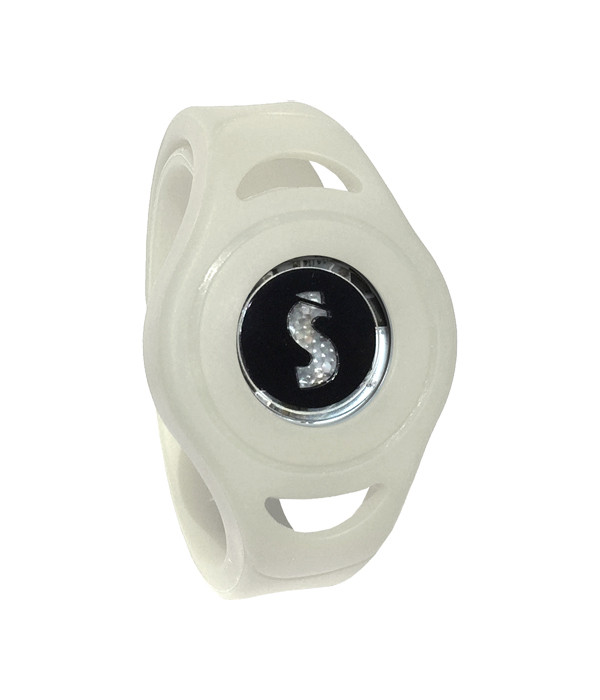
\includegraphics[scale=0.31]{figures/aProblemanalyse/sqord.JPG}
	\caption{På figuren ses The Sqord Booster sat i et armbånd. \citep{Sqord2016}}
	\label{fig:sqord}
\end{figure}
%Hjemmesiden hvor børnene kan følge med i deres avatar, fungerer som et forum, hvor de har mulighed for at give hinanden highfives for gode præstationer, chatte indbyrdes, eller lave talebobler, hvor alle kan se hvad de skriver. \citep{Sqord_family2015} \newline
The Sqord Booster tilgodeser alle præstationer, idet alle får en medalje ved at have deltaget i en given aktivitet. Vinderen får imidlertid flere point end de andre deltagere. Spillet er designet således, at alle har mulighed for at vinde. Dette er muligt, da der i det enkelte spil vurderes ud fra børnenes individuelle form igennem tidligere præstationer. \citep{Sqord_family2015} \newline
The Sqord Booster har endvidere en indkøbspris på 230 kr \citep{Sqord_family2015}. 

\subsubsection{Vurdering af succeskriterier}
Aktivitetsmåleren registrerer børnenes aktivitet ved gang og løb men kan ikke skelne mellem aktiviteterne og der registreres ikke cykling. Der måles ikke intensitet af det udførte arbejde, da dette ikke kan lade sig gør ved hjælp af et accelerometer.\\ %idet den indbyggede sensor ikke kvalificerer sig til dette. %  kun accelerometerets fart vurderes. \newline
Børnene bliver aktiveret socialt, da hjemmesiden er en blanding mellem et chatforum og en oversigt over præstationer. Derudover har børnene mulighed for at konkurrere med og mod hinanden. The Sqord Booster henvender sig både til inaktive og aktive børn, da alle har mulighed for at vinde. Aktivitetsmåleren er mulig at placere flere steder, hvormed børnene har mulighed for at vælge en placering, hvor det er til mindst gene.~\citep{Sqord_family2015,Sqord_group2015}\fxnote{Derudover er det designet efter målgruppen, hvormed aktivitetsmåleren både kan modstå stød og tåle at komme i vand.}

The Sqord Booster opfylder to ud af seks succeskriterier, mens det delvist opfylder to succeskriterier.

\subsection{Nabi Compete}
Nabi Compete er en aktivitetsmåler, som appellerer til børn over seks år gennem deres madvaner og samvær med andre. Der er muligt for børnene at konkurrerer individuelt, men hovedformålet er at konkurrere andre som et hold. Konkurrencerne kan bestå i at løbe en bestemt rute, som børnene selv kan designe og tegne ind. Desuden kan børnene vælge en fødevare i brugerfladen, som kan informere børnene om, hvor meget fysisk aktivitet der kræves for at forbrænde denne fødevare. Herved kan der opstå konkurrence i at forbrænde flest kalorier eller løbe længst. %Det er muligt at opnå mål sammen med andre, eller dyste i hvem der når forskellige mål først. 
\fxnote{Derudover lærer børnene om kalorier og distance ved at bruge appen, hvor det er muligt at følge med i progressionen.} Gennem konkurrencerne optjenes der point, som kan bruges til at købe et virtuelt dyr, der udvikles ved hjælp af point. 
Aktiviteten måles gennem et tre-akse accelerometer, som sidder i et armbånd, hvilket kan ses på \figref{fig:nabi}. Dataet synkroniseres til en app gennem bluetooth, hvor der kan gemmes data i op til 90 dage. Barnet og forældrene har dermed mulighed for at følge med i barnets progression. 
Nabi Compete har endvidere en indkøbspris på 190 kr \citep{Fuhu2015,Fuhu_tech2015}. 

\begin{figure}[H]
	\centering
	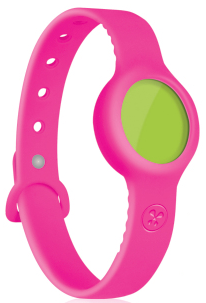
\includegraphics[scale=0.8]{figures/aProblemanalyse/nabi.png}
	\caption{På figuren ses Nabi Compete. \citep{Perez2015}}
	\label{fig:nabi}
\end{figure}

\subsubsection{Vurdering af succeskriterier}
Aktivitetsmåleren registrer gang og løb, men det er ikke muligt at skelne mellem aktivitetsformerne. Der registreres heriblandt ikke cykling eller intensitet. Børnene aktiveres socialt, da appen er designet med mulighed for at konkurrere mod hinanden eller arbejde sammen i hold. Derudover har børnene mulighed for %at have et kæledyr på appen, hvorved de, %udover at konkurrere mod andre, kan 
at se, hvor mange kalorier de har forbrændt. Aktivitetsmåleren er designet som et armbånd med en justerbar rem, hvilket gør at den kan monteres og placeres på komfortabel vis.~\citep{Fuhu2015,Fuhu_tech2015}\fxnote{Derudover er den designet således at den kan tåle sved og regn, hvilket gør at børnene kan bruge det i al slags vejr.}

Nabi Compete opfylder to ud af seks succeskriterier, mens det delvist opfylder to succeskriterier.

\subsection{Ibitz}
Ibitz er en aktivitetsmåler, som appellerer til børn over fem år gennem udfordringer i samarbejde med forældrene. Ibitz har generelle udfordringer inkorporeret, men designet opfordrer især til, at forældrene skal sætte målene for børnene. Forældrene har mulighed for at lave en række opgaver til deres børn, som de vurderer er passende i forhold til barnets aktivitetsniveau. \newline
Disse udfordringer kan indebære, hvor meget tid børnene skal bruge på en aktivitet. Ved at gennemføre udfordringerne, kan børnene optjene point, der kan bruges på to forskellige elektroniske spil. \newline
%Dette kan være for hvornår der er legetid, hvornår de må sidde foran skærmen eller hvornår de skal lave aktiviteter med forældrene. 
Aktivitetsmåleren består af et pedometer, som måler skridt, der trådløst synkroniseres med en app via bluetooth. Appen gemmer aktiviteterne i 30 dage, hvorved barnet og forældrene har mulighed for at følge med i progressionen. Aktivitetsmåleren monteres ved en klemme, som det fremgår af~\figref{fig:ibitz}, og har endvidere en indkøbspris på 165 kr. \citep{Ibitz_features2016}

\begin{figure}[H]
	\centering
	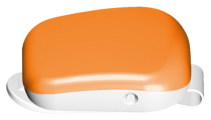
\includegraphics[scale=0.9]{figures/aProblemanalyse/ibitz.png}
	\caption{På figuren ses Ibitz klemmen.\citep{Ibitz_features2016}}
	\label{fig:ibitz}
\end{figure}

\subsubsection{Vurdering af succeskriterier}
Aktivitetsmåleren registrer gang og løb, men der er ikke muligt at skelne mellem aktivitetsformerne eller registrere intensitet samt cykling. Børnene bliver delvist aktiveret socialt, hvor det primært er sammen med familien. Derudover aktiveres børnene ved at tjene point til forskellige spil, som oftest spilles sammen med andre børn. Aktivitetsmåleren monteres uden gene, da børnene selv kan vælge mellem at montere den på buksen eller skoen.\fxnote{Derudover kan den tåle vand, hvorved børn også kan bruge den i regnvejr}  

Ibitz opfylder to ud af seks succeskriterier, mens det delvist opfylder to succeskriterier.

\subsection{Samlet vurdering af de udvalgte aktivitetsmålere}
Ovenstående analyse og vurdering af de udvalgte aktivitetsmålere viser, at ingen af aktivitetsmålere opfylder alle de opstillede succeskriterier. \newline
Fælles for aktivitetsmålerne er, at alle kan registrere løb og gang, men de kan ikke automatisk adskille disse aktivitetsformer. Yderligere var ingen af aktivitetsmålerne i stand til at registrere intensitet eller cykling. Det er vurderet, at alle aktivitetsmålerne har en motiverende elementer således, at disse henvender sig til både fysisk aktive og inaktive børn. Desuden kan alle aktivitetsmålerne monteres og placeres på komfortabel vis, således børnene ikke oplever gener ved at benytte dem. Indkøbsprisen for den enkelte aktivitetsmåler fremgår af nedenstående tabel. Denne pris vil kunne benyttes til at vurdere og sammenligne effektiviteten og prisen for de udvalgte aktivitetsmålere.  

%Ud fra vurderingen ses det, at de aktivitetsmålere, der i dag benyttes til børn i projektets aldersgruppe, ikke lever op til samtlige af de succeskriterier, som er stillet. De kan alle registrere løb og gang men har ikke mulighed for at skelne mellem de to aktivitetsformer. Ingen af aktivitetsmålerne registrerer cykling eller intensitet. Alle aktivitetsmålerne appellerer til både inaktive og aktive børn. Alle aktivitetsmålere er beregnet til at have rundt om armen, hvor den spændes på med en justerbar rem. Derudover er alle aktivitetsmålere designet efter, at børnene både skal kunne bruge dem i såvel regnvejr som solskin.

\begin{table}[H]
	\centering
	\resizebox{\textwidth}{!}{%
		\begin{tabular}{l c c c c}
			\rowcolor[HTML]{C0C0C0} 
			\multicolumn{1}{c}{\cellcolor[HTML]{C0C0C0}Krav} & \multicolumn{1}{c}{\cellcolor[HTML]{C0C0C0}Unicef Kid Power Band} & \multicolumn{1}{c}{\cellcolor[HTML]{C0C0C0}Sqord Booster}    &    \multicolumn{1}{c}{\cellcolor[HTML]{C0C0C0}Nabi Compete}     &   \multicolumn{1}{c}{\cellcolor[HTML]{C0C0C0}Ibitz} \\
			Registrere gang                                 & (x)                                        & (x)                                & (x)                               & (x)                        \\ \hline
			Registrere løb                                  & (x)                                        & (x)                                & (x)                               & (x)                        \\ \hline
			Registrere cykling                              &                                            &                                    &                                   &                            \\ \hline
			Registrere intensitet              &                                            &                                    &                                   &                            \\ \hline
			Motivere inaktive såvel som aktive børn         & x                                          & x                                  & x                                 & x                          \\ \hline
			Monteres uden gene                              & x                                          & x                                  & x                                 & x                          \\ \hline
			Pris                                 & 280 kr.                                        & 230 kr.                               & 190 kr.                               & 165 kr.                      \\ \hline
		\end{tabular}
	}
	\caption{Tabellen viser en oversigt over de fire aktivitetsmålere, samt hvorvidt de lever op til succeskriterierne. (x) betyder, at de delvist lever op til succeskriterierne. x betyder, at de lever op til succeskriterierne}
	\label{tab:sammenhold_tracker}
\end{table}\vspace{-0.5cm}
For at optimere de aktivitetsmålere, der benyttes i dag, vurderes det, at de skal være i stand til at skelne mellem gang, løb og cykling. Barnet kan derved både få overblik over dagens totale fysiske aktivitetsniveau, da al aktivitet herigennem bør registreres. %skal de kunne skelne mellem løb, gang og cykling, så barnet ikke kun kan måle, hvor mange skridt vedkommende har gået, eller hvor langt de er nået men også kan måle hvilken aktivitet, som er udført. 
Derudover vurderes det, at det vil være optimalt, hvis intensiteten af den fysiske aktivitet kan registreres ved hjælp af puls. Denne er sigende for det fysiologiske udbytte af den givne aktivitet, hvilket kan ses på \tabref{tab:PA_Procentpuls} i \secref{subsub:ak_int}.\newline
Aktivitetsmåleren skal aktivere børnene socialt sammen med andre børn. Derudover skal aktiviteterne foregå igennem leg eller spil, som både skal være baseret på konkurrence mod andre eller sammenspil i hold.